\section{Distributed Processing}

Um die Belastung der Host-CPU zu reduzieren sollen Audio-Verarbeitungsaufgaben an externen SBCs über Gigabit-Ethernet verteilt werden. Auf der Host-CPU arbeitet der  Audio Plug-in als Master-Knoten. Für den Host-DAW, sollte die Verteilung der Audio-Verarbeitungsaufgaben vollkommen unsichtbar sein. Der Master-Knoten empfängt, MIDI- und Audiodaten von der Host-DAW und gibt die Ergebnisse zurrück wie jede andere Audio-Plugin.

Das Plug-in bekommt Zugriff auf eine kleine Puffer Audiodaten, in sehr kurze regelmässigen Abständen. Das Plugin muss in kurzer Zeit die Daten verarbeiten und zurück an das Host DAW-Anwendung, bevor der nächste Puffer bereitsteht. Dies stellt einige Grenzen, wie Bearbeitungsaufträge verteilt werden kann.

Es gibt verschiedene Arten Verarbeitungsaufgaben zu parallelisieren. Jedes Plug-in-Instanz könnte den gesamten Auftrag an einem Rechenknoten delegieren wie in Abbildung \ref{fig:one_to_one} dargestellt. Besteht einer Verarbeitungsaufgaben aus mehreren, in serie geschalteten, Verarbeitungsblöcke, dann könnte jedes Block einen Rechenknoten zugeteilt werden, wie in Abbildung \ref{fig:perproccessor} dargestellt. Speziell bei einer Virtuellen-Synthesizer-Plug-in könnte jede gespielte Stimme seinem eigenen Rechenknoten zugeteilt werden, wie in Abbildung \ref{fig:pervoice} dargestellt.


\begin{figure}[H]
    \centering
    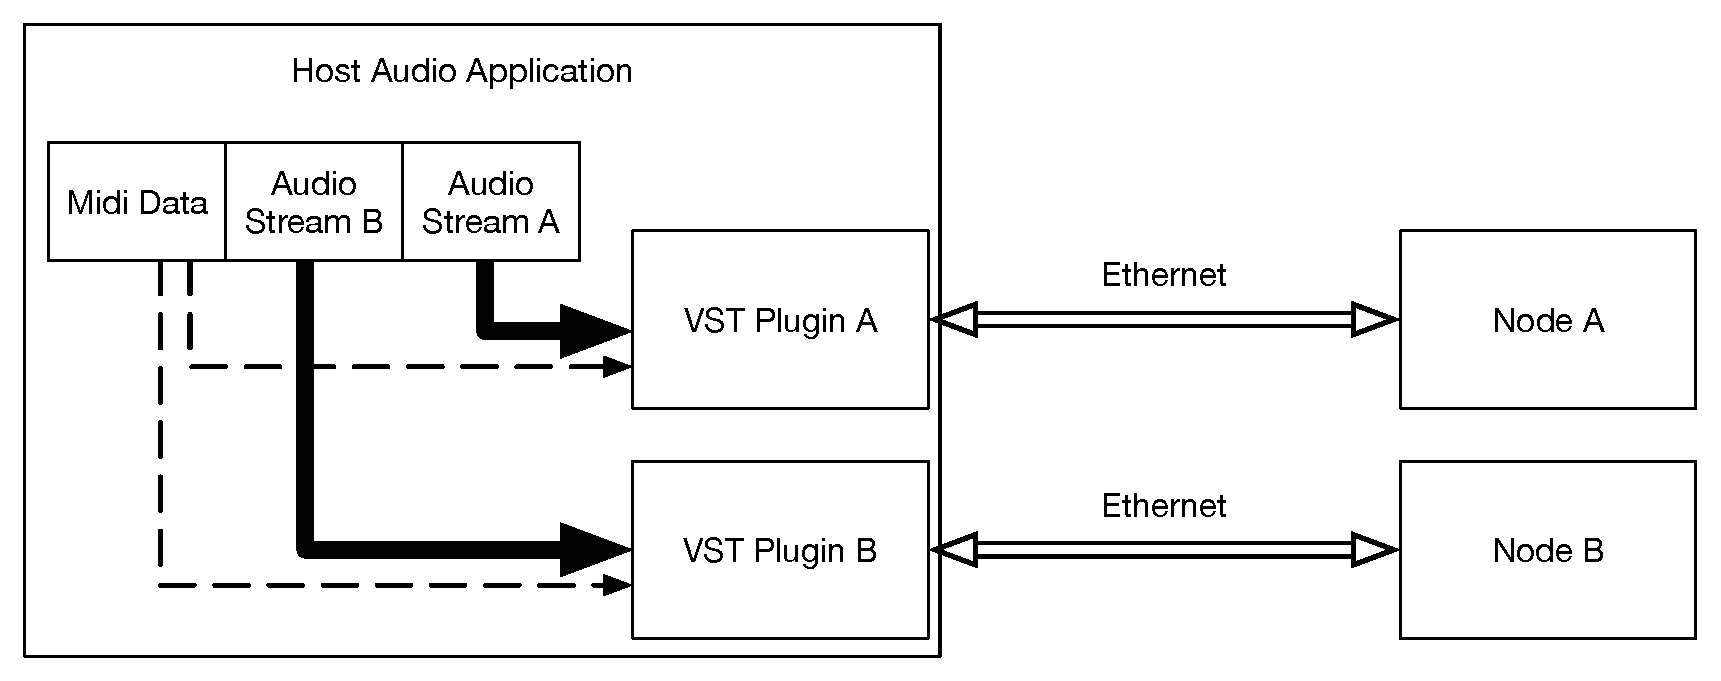
\includegraphics[width=\textwidth]{assets/distribution_1to1.pdf}
    \caption{Jedes Plugin Verteilt an einen Knoten}
    \label{fig:one_to_one}
\end{figure}

\begin{figure}[H]
    \centering
    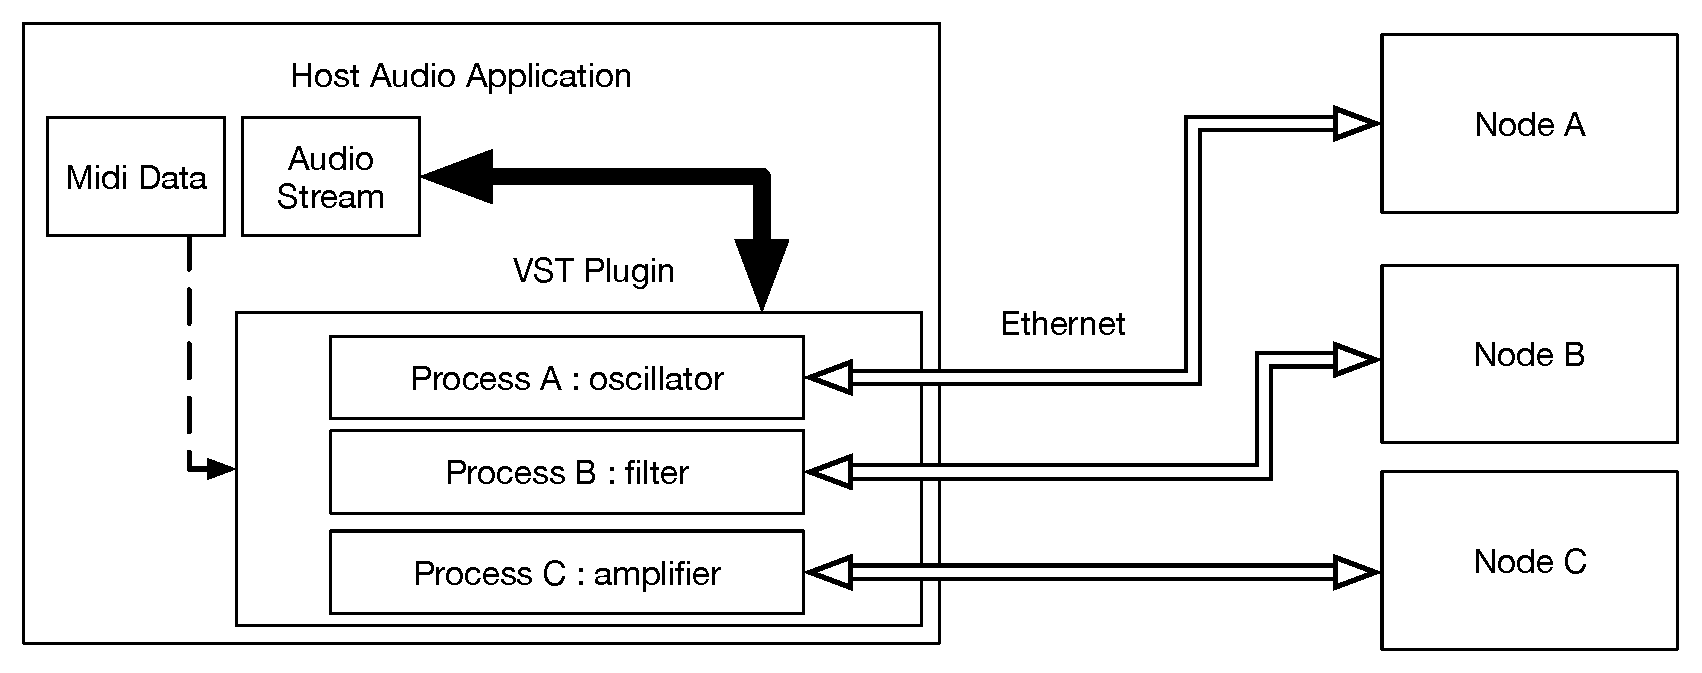
\includegraphics[width=\textwidth]{assets/distribution_perprocessor.pdf}
    \caption{Jeder Verarbeitungsblock Verteilt an einen Knoten}
    \label{fig:perproccessor}
\end{figure}

\begin{figure}[H]
    \centering
    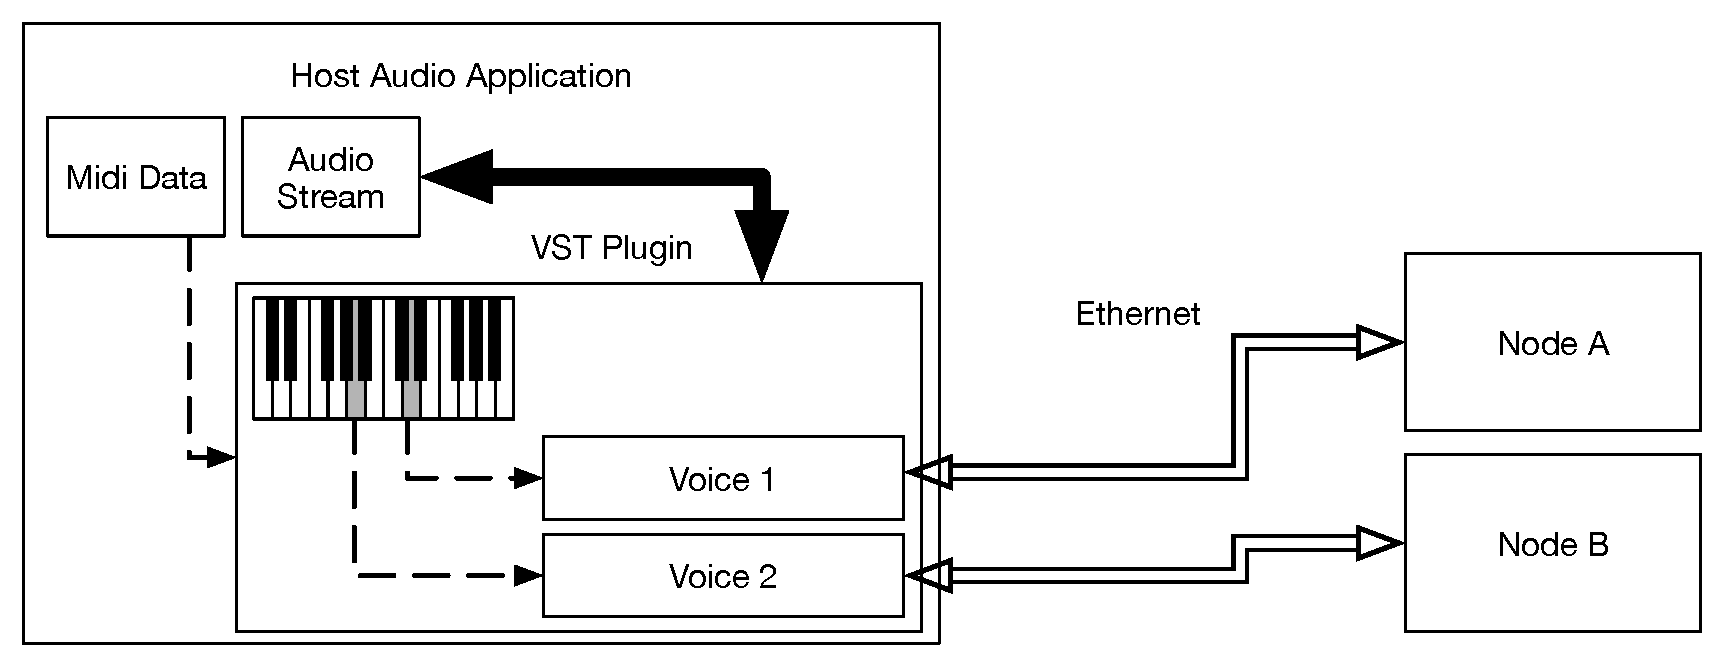
\includegraphics[width=\textwidth]{assets/distribute_byvoice.pdf}
    \caption{Jedes Synth Stimme Verteilt an einen Knoten}
    \label{fig:pervoice}
\end{figure}

Für dieses Projekt wird die zweite Option implementiert aus Testbarkeitsgründen, auch wenn es vielleicht nicht der effizienteste Implementierung ist.